\section{Metodología}
\subsection{Figuras}
Las preocupaciones son mucho mayores cuando se trabaja fuera, por no hablar de las molestias propias de los viajes: estar pendiente de los enlaces de los trenes; la comida mala, irregular; relaciones que cambian constantemente, que nunca llegan a ser verdaderamente cordiales, y en las que no tienen cabida los sentimientos. ¡Al diablo con todo!

Se puede ver en más detalle en la \autoref{fig:propuesta}.

\begin{figure}[h]
	\centering
	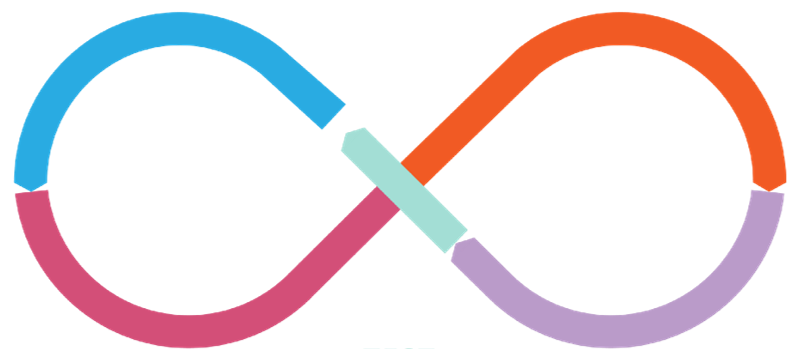
\includegraphics[width=0.65\linewidth]{process}
	\caption{Imagen inicial de la propuesta del cliente.}
	\label{fig:propuesta}
\end{figure}

También se puede poner dos subfiguras dentro de la definición de una figura (\autoref{fig:doble}), lo cual puede ser útil para hablar de dos gráficas relacionadas o algo similar. 

\begin{figure}[h!]
	\centering
	\begin{subfigure}{.45\textwidth}
		\centering
		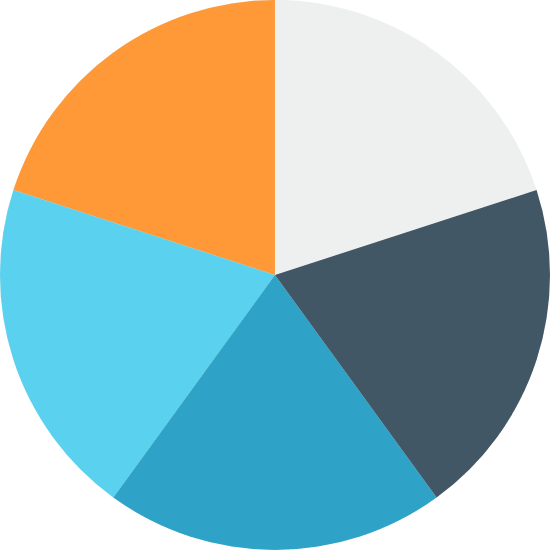
\includegraphics[width=1.7in]{pie_chart}%
		\caption{Una torta.}
		\label{fig:torta}
	\end{subfigure} 
	\hfil
	\begin{subfigure}{.45\textwidth}
		\centering
		
\includegraphics[width=1.7in]{bar_chart}%
		\caption{Unas barras}
		\label{fig:barras}
	\end{subfigure}
	\caption{Este es un caso en donde se pueden poner dos imágenes juntas, se tiene la \autoref{fig:torta} y por otro lado se tiene la \autoref{fig:barras}.}
	\label{fig:doble}
\end{figure}

Una mañana, tras un sueño intranquilo, Gregorio Samsa se despertó convertido en un monstruoso insecto. Estaba echado de espaldas sobre un duro caparazón y, al alzar la cabeza, vio su vientre convexo y oscuro, surcado por curvadas callosidades, sobre el que casi no se aguantaba la colcha, que estaba a punto de escurrirse hasta el suelo.

Sobre la mesa había desparramado un muestrario de paños - Samsa era viajante de comercio-, y de la pared colgaba una estampa recientemente recortada de una revista ilustrada y puesta en un marco dorado. La estampa mostraba a una mujer tocada con un gorro de pieles, envuelta en una estola también de pieles, y que, muy erguida, esgrimía un amplio manguito, asimismo de piel, que ocultaba todo su antebrazo.

\subsubsection{Descripción del equipo}

\begin{wrapfigure}[9]{l}{0.3\linewidth} % Poner cantidad de lineas, alineación y ancho de la hoja
	\vspace{-17pt}
	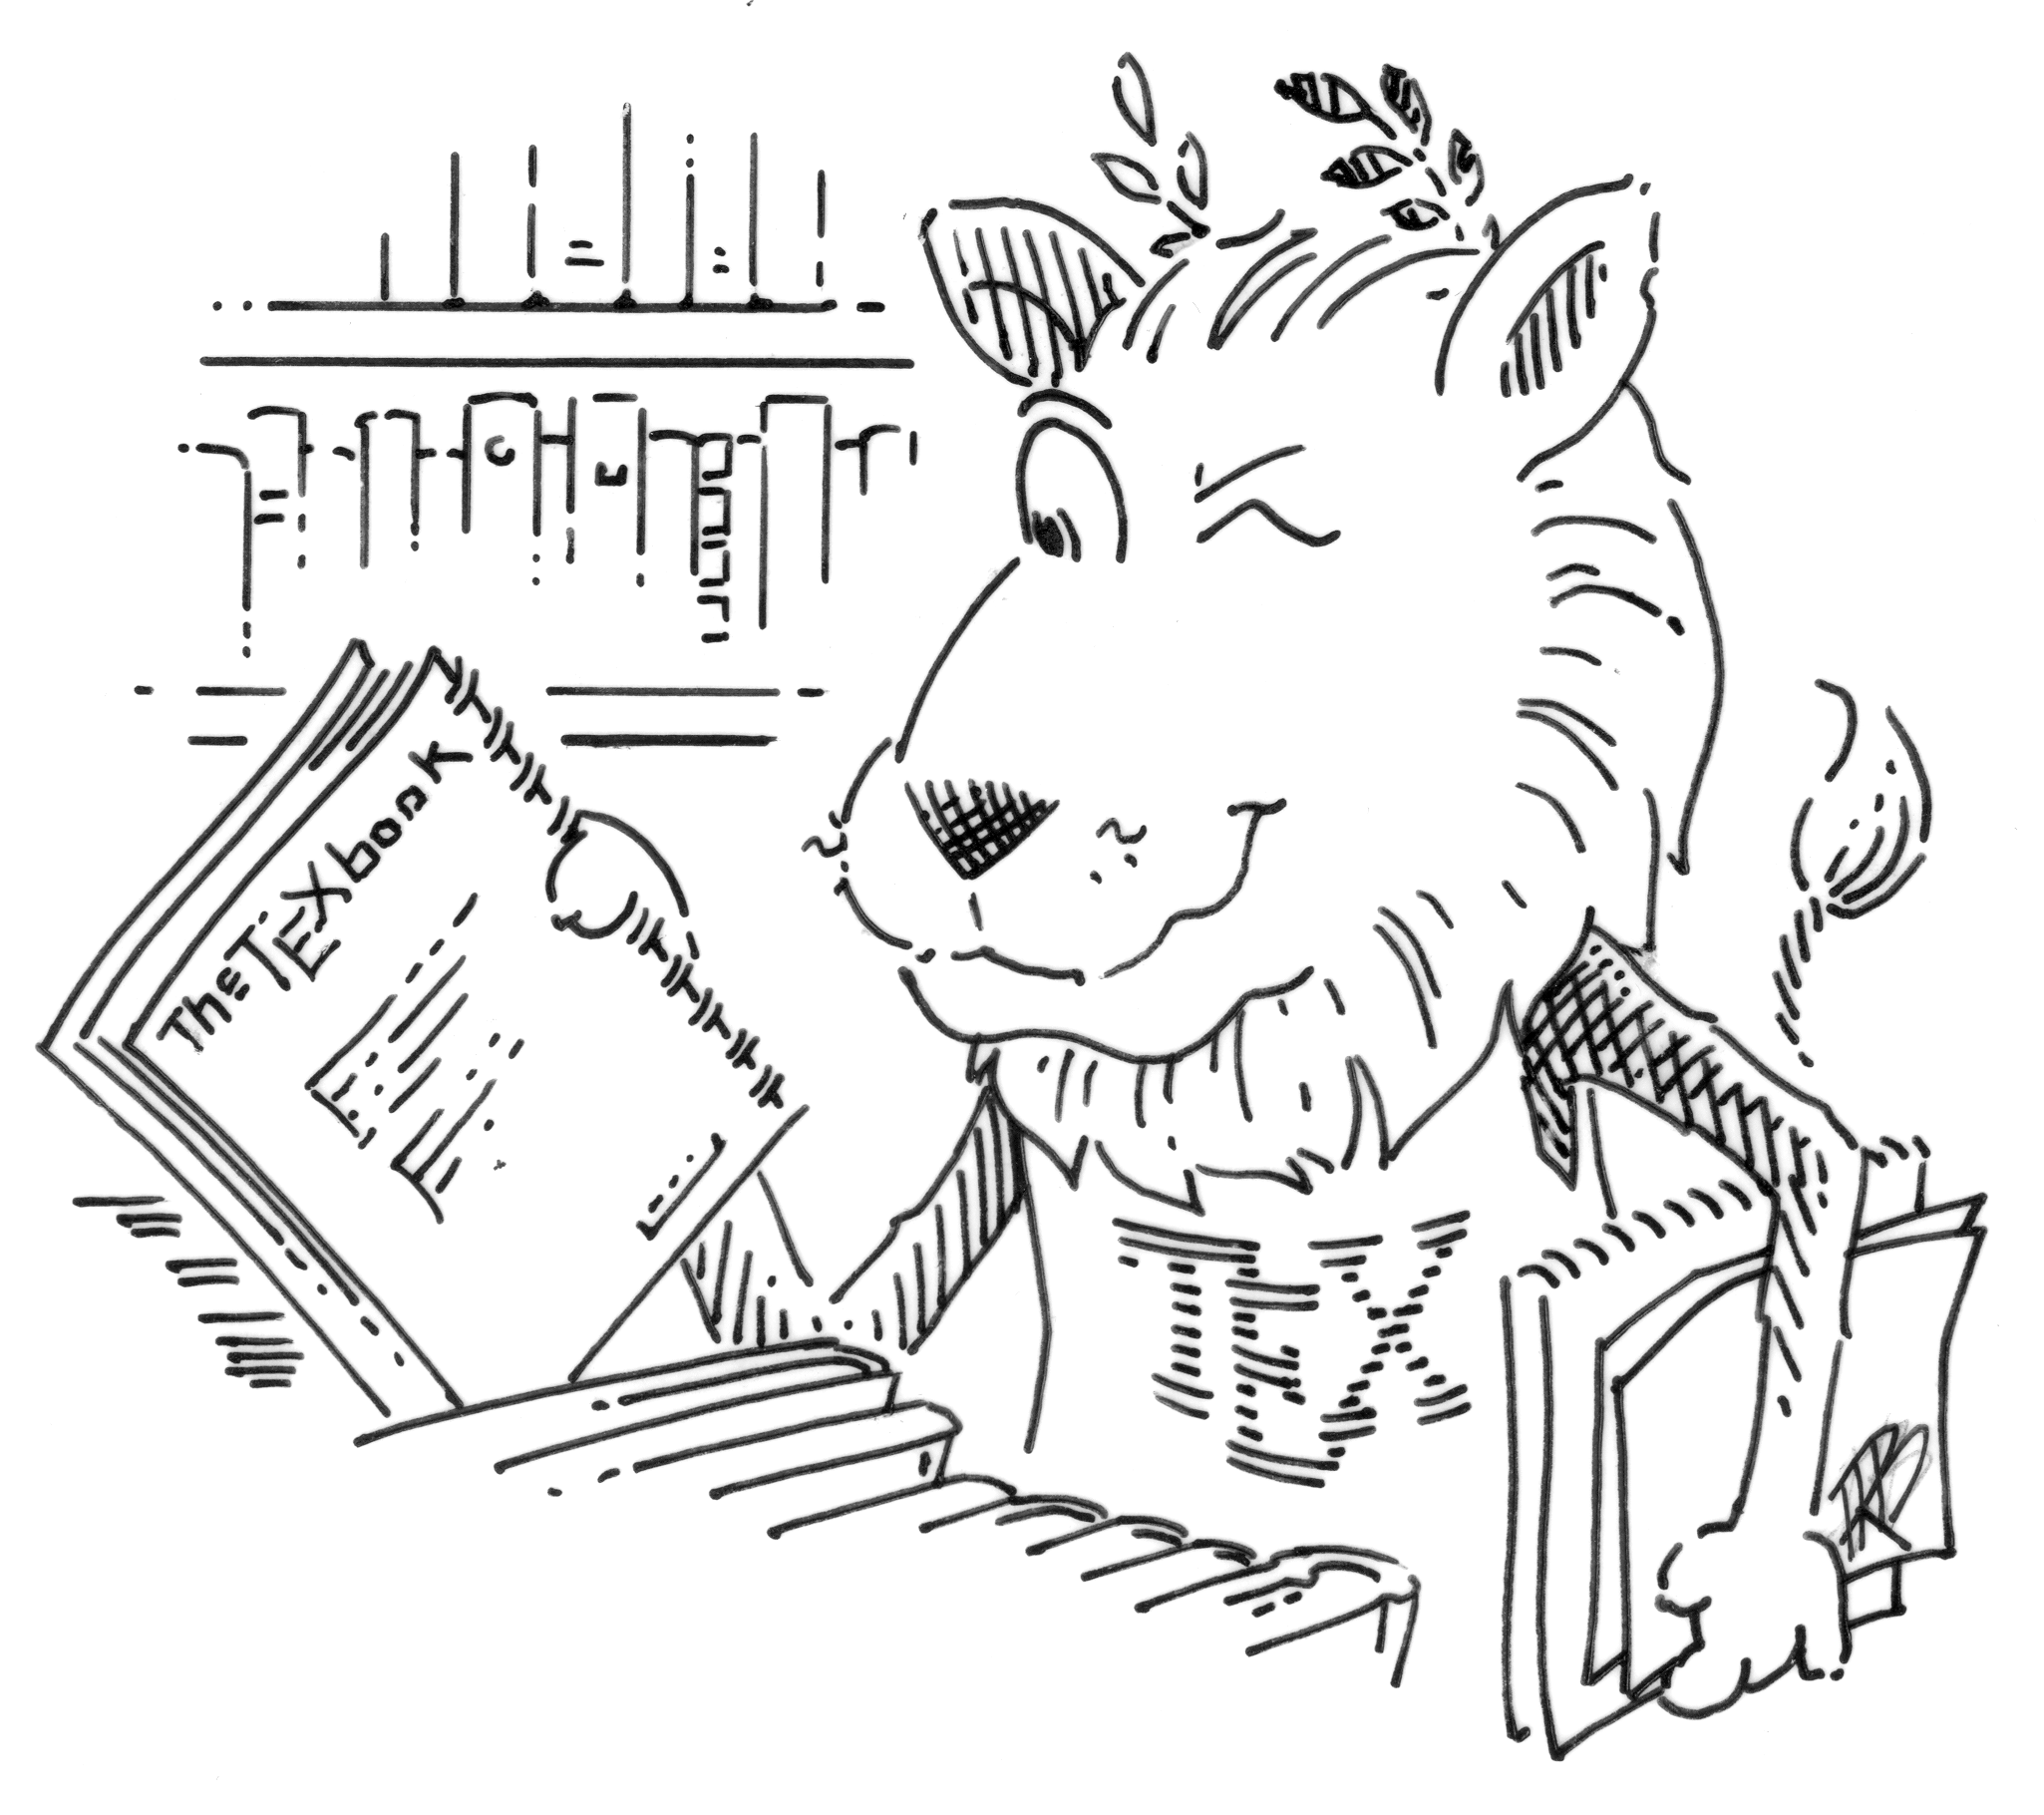
\includegraphics[width=1\linewidth]{tex_lion}
\end{wrapfigure}

\noindent {\large \textbf{\textcolor{blue}{El león de \TeX}}}\\ [5pt]
	% Notar que el texto a colocar al lado de la figura debe estar debajo del entorno wrapfigure

Gregorio miró hacia la ventana; estaba nublado, y sobre el cinc del alféizar repiqueteaban las gotas de lluvia, lo que le hizo sentir una gran melancolía. «Bueno -pensó-; ¿y si siguiese durmiendo un rato y me olvidase de todas estas locuras? » Pero no era posible, pues Gregorio tenía la costumbre de dormir sobre el lado derecho, y su actual estado no le permitía adoptar tal postura.

Por más que se esforzara volvía a quedar de espaldas. Intentó en vano esta operación numerosas veces; cerró los ojos para no tener que ver aquella confusa agitación de patas, que no cesó hasta que notó en el costado un dolor leve y punzante, un dolor jamás sentido hasta entonces. - ¡Qué cansada es la profesión que he elegido! -se dijo-. Siempre de viaje.

\subsubsection{Gráfico importante}

Esto sería un gráfico importante, como el de la \autoref{fig:grafico}.

\begin{figure}[h!]
	\centering
	\begin{overpic}[width=0.6\textwidth,tics=5]{Plot} % Poner ",grid" luego de tics para activar la grilla. "tics" es la separación en la grilla.
		\put (20,01) { 5 }
		\put (40,01) { 10 }
		\put (60,01) { 15 }
		\put (80,01) { 20 }
		\put (-2,20) { 5 }
		\put (-2,40) { 10 }
		\put (-2,60) { 15 }
		\put (63,67) {$\boxed{ f(x) = x^3 }$} % Ponerlo al ver ecuaciones
	\end{overpic}
	\caption{El camino del éxito.}
	\label{fig:grafico}
\end{figure}
\subsection{Tablas}
Numerosas patas, penosamente delgadas en comparación con el grosor normal de sus piernas, se agitaban sin concierto. - ¿Qué me ha ocurrido? No estaba soñando. Su habitación, una habitación normal, aunque muy pequeña, tenía el aspecto habitual. 

\begin{center}
	\begin{tabular}{|l|c|c|c|}
		\hline   & 1 & 2 & 3 \\ 
		\hline A &  &  &  \\ 
		\hline B &  &  &  \\ 
		\hline 
	\end{tabular} 
\end{center}

Podemos hacer una tabla con un poco más de estilo, con ecuaciones dentro
y que se adapte el texto.
Para el Estado Límite de Servicio, los coeficientes parciales de seguridad a adoptar son los indicados en la \autoref{tab:coeficientes}.\footnote{\textcolor{grayblack}{Justo está bueno poner una nota al pie por acá.}}

\begin{table}[h]
	\centering
	\caption{Coeficientes parciales de seguridad en ELS.}
	\arrayrulecolor{grayblack}
	\rowcolors{1}{white}{gray}
	{\color{grayblack}
	\begin{tabular}{p{4cm}cc}
		\toprule
		\textbf{Tipo de acción}    & \textbf{Efecto desfavorable} & \textbf{Efecto favorable}\\
		\midrule
		Permanente & $\gamma_G=1.00$ & $\gamma_G=1.00$ \\
		Pretensado & 1.10 & 0.9 \\
		Permanente de valor no constante  & 1.00 & 1.00 \\
		Variable & 1.00 & 0.00 \\
		\bottomrule
	\end{tabular}}
	\label{tab:coeficientes}
\end{table}%

Sintió en el vientre una ligera picazón. Lentamente, se estiró sobre la espalda en dirección a la cabecera de la cama, para poder alzar mejor la cabeza. Vio que el sitio que le picaba estaba cubierto de extraños untitos blancos. Intentó rascarse con una pata; pero tuvo que retirarla inmediatamente, pues el roce le producía escalofríos.

El cronograma preliminar se presenta en la \autoref{tab:cronograma}.
	
\begin{table}[h]
	\centering
	\caption{Cronograma tentativo.}
	{\color{grayblack}
	\begin{tabular}{p{2.2em}p{14em}lllr}
		\multicolumn{1}{l}{} & \multicolumn{1}{r}{} & \multicolumn{4}{c}{\textbf{2022}} \\
		\midrule
		\textbf{Etapa} & \textbf{Productos/Entregables} & \multicolumn{1}{p{4.055em}}{\textbf{Ene-Mar}} & \multicolumn{1}{p{4.055em}}{\textbf{Abr-Jun}} & \multicolumn{1}{p{4.055em}}{\textbf{Jul-Set}} & \multicolumn{1}{p{4.055em}}{\textbf{Oct-Dic}} \\
		\midrule
		E1    & Primer documento a entregar, en .doc. &       & \cellcolor[rgb]{ .718,  .871,  .91} &       &  \\
		E2    & Segundo documento, más pesado. & \cellcolor[rgb]{ .776,  .89,  .859} &       &       &  \\
		E2    & Este tema mejor que no falte. &       & \cellcolor[rgb]{ .776,  .89,  .859} &       &  \\
		E2    & Otro tema interesante en PDF. &       &       & \cellcolor[rgb]{ .776,  .89,  .859} &  \\
		E2    & Esto es importante, también va. &       &       & \cellcolor[rgb]{ .776,  .89,  .859} &  \\
		E3    & Un documento para ver como vamos, editable. &       & \cellcolor[rgb]{ .722,  .804,  .894} &       &  \\
		E4    & Informe de evaluación hasta ahora. &       & \cellcolor[rgb]{ .722,  .804,  .894} &       &  \\
		E5    & Diseño final del sistema. &       &       &       & \cellcolor[rgb]{ .722,  .804,  .894} \\
		E6    & Recomendaciones estratégicas. &       &       &       & \cellcolor[rgb]{ .722,  .804,  .894} \\
		\bottomrule
	\end{tabular}}
	\label{tab:cronograma}%
\end{table}%


\subsection{Ecuaciones}
Vamos a poner un poco de texto acá para que se note que sabemos lo que decimos. La ecuación $ E=m\cdot c^2 $. Tenemos $ f_{yk} $ o sino $ x_{a}^{2} $. También tenemos $ \frac{2}{4} $ o sino $ \dfrac{3}{4} $ o la raíz $ \sqrt{2} $.

$$ E=m\cdot c^2 $$

Como vimos en la ecuación \ref{eq:energía}. La \autoref{eq:energía} o sino la ecuación \eqref{eq:energía}.
\begin{equation} \label{eq:energía}
	E=m\cdot c^2
\end{equation}

Otra opción es una ecuación sin numerar pero dentro del entorno de ecuaciones:
\begin{equation*} \label{eq:energía2}
	E=m\cdot c^2
\end{equation*}

La suma es $ a+b $ y la resta $ a-b $. Multiplicación es $ a\cdot b$ o si no $ a \times b $. Si estoy con ángulos puedo tener $ \cos(30) $ o si no $ \sin(45) $. Una integral:
$$ \int_0^L x^2, \quad 10<15 \Rightarrow 15 \geq 10$$

Lista de ecuaciones alineadas
\begin{align}
	f(x) &= x^2+x^3			\\
	&= x^2+x^2\cdot x 
\end{align}
\begin{align*}
	f(x) &= x^2+x^3			\\
	&= x^2+x^2\cdot x 
\end{align*}
Matrices
\begin{equation*}
	A = 
	\begin{pmatrix}
		1 & 2 & 3 \\
		4 & 5 & 6 \\
		7 & 8 & 9
	\end{pmatrix}, \quad
	B = 
	\begin{bmatrix}
		1 & 2 & 3 \\
		4 & 5 & 6 \\
		7 & 8 & 9
	\end{bmatrix}, \quad
	C =
	\begin{matrix} 
		a_{11} & a_{12}  \\
		a_{21} & a_{22}  
	\end{matrix}, \quad
	D = 
	\begin{Bmatrix} 
		a_{11} & a_{12}  \\
		a_{21} & a_{22}  
	\end{Bmatrix} 
\end{equation*}
